\chapter{Particle Physics}
\label{chap:particlephysics}

Particle physics is the study of the elementary particles and fundamental forces
of nature. By ``elementary particles'' we mean the smallest, most
basic building blocks of all structures in the universe. By
``fundamental forces'' we mean the basic kinds of interactions between
particles, from which all other possible interactions in the universe
arise.

This chapter will provide a basic introduction to the terminology
and principles of particle physics, with the goals of motivating the
research in this dissertation, and also making it understandable to
readers outside the particle physics community.

\section{The Standard Model}
\label{sec:standardmodel}

\subsection{Description}
\label{ssec:SMdescription}

The Standard Model (SM) is the scientific theory that describes
(almost) all the particles and forces we know of and their properties.
It is a relativistic quantum field theory, describing both the
behavior of particles at speeds up to (and including) the speed of
light, as well as their quantum mechanical nature.
The SM was developed over several decades of the 20\textsuperscript{th}
century through the joint efforts of theoretical and experimental physicists.
Although it is not a perfect description of all known phenomena in
particle physics, it is still widely considered to be one of the most
successful scientific theories of all time. %Citation?

The Standard Model describes two families of matter particles--that is
to say, particles that give rise to tangible materials at the macro scale.
These two families are called quarks and leptons. In addition, it
describes several force-carrying particles, as well as the Higgs
boson. A sort of ``periodic table'' of these particles is given in
Figure \ref{fig:standardmodel}. A diagram showing which particles
interact with which other particles is given in Figure \ref{fig:couplings}.

\begin{figure}[h]
  \centering
  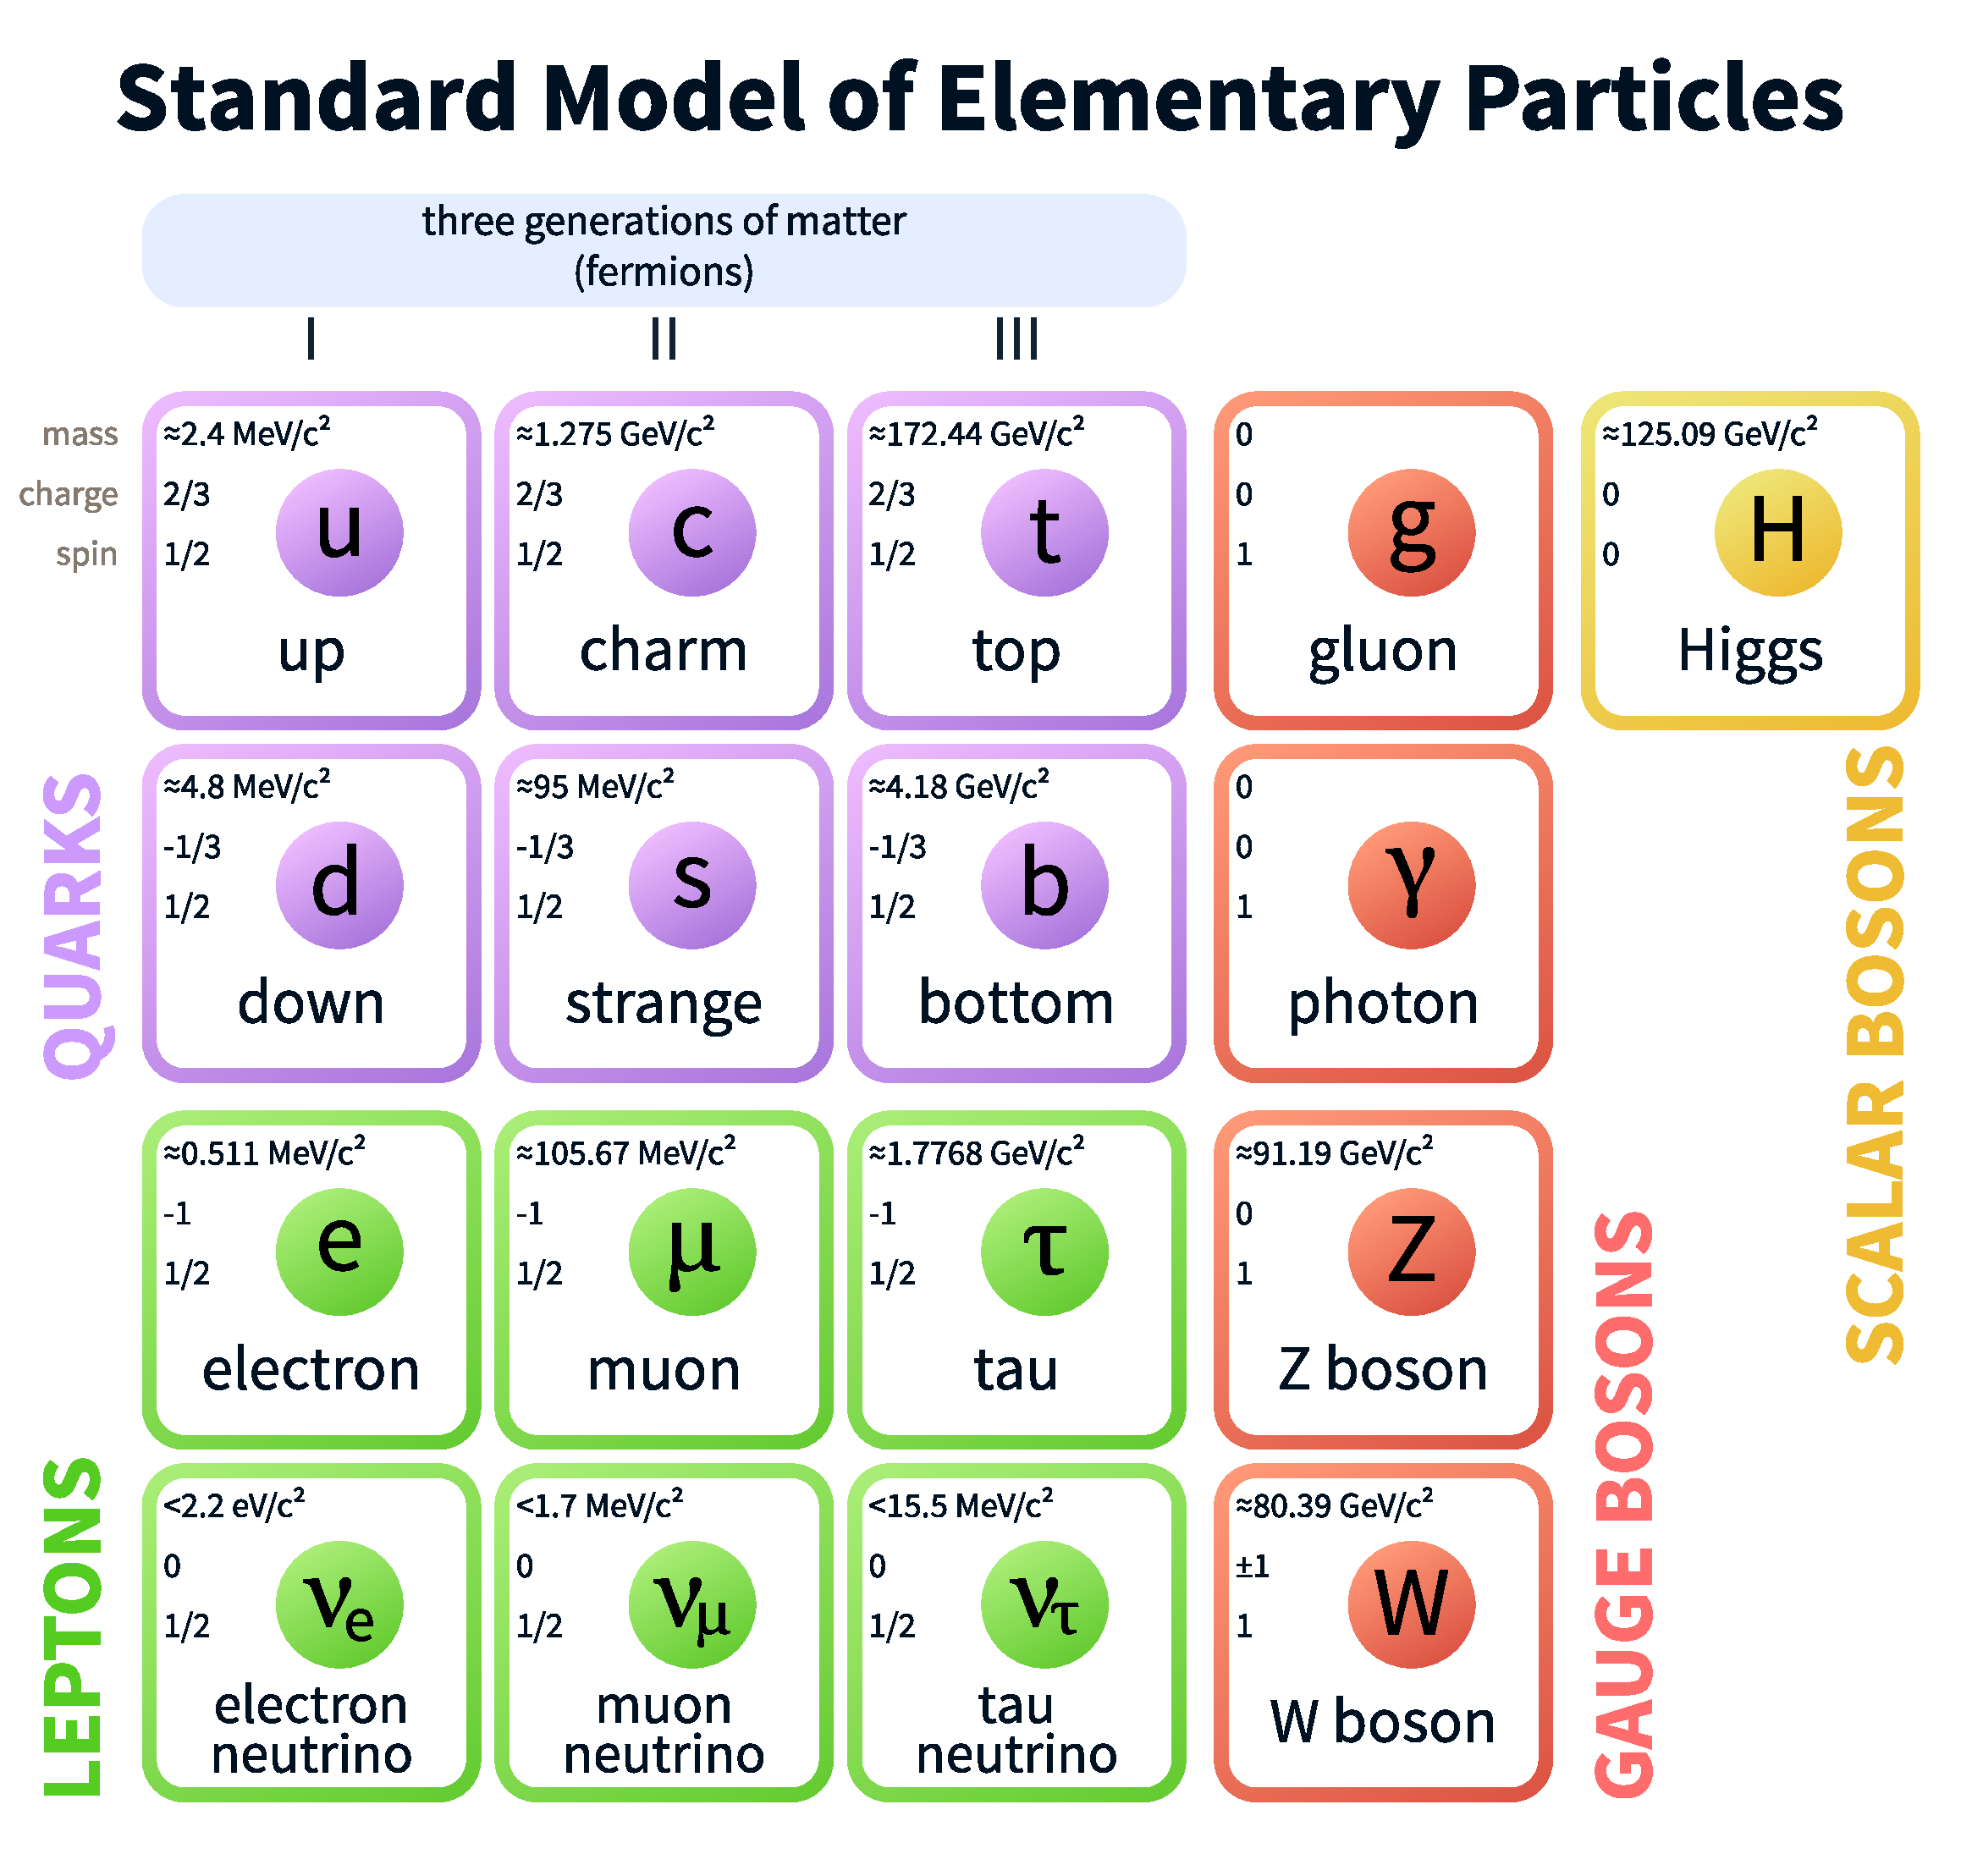
\includegraphics[width=0.75\textwidth]{figures/standard-model-light.pdf}
  \caption%[A diagram of all the particles of the Standard Model,
          %grouped into families of related particles.]
  {A diagram of all the particles of the Standard Model, grouped into
  families of related particles. Mass measurements are constantly
  being improved, and the listed mass values may not reflect the latest and
  best measurements.}
  \label{fig:standardmodel}
\end{figure}

\subsubsection*{Quarks}
There are six quarks in the SM. In order from lightest to heaviest,
these quarks are named \emph{up, down, strange, charm, bottom,} and
\emph{top}. They are often referred to using only the first letter of
their names. The up and down quarks are essential to our lives, as
they make up the nuclei of atoms. The proton is composed of two up
quarks and a down quark bound together ($uud$), and the neutron is composed of one up
quark and two down quarks ($udd$) bound together. The four heavier
quarks tend to decay into lighter quarks within a fraction of a
second, so they're generally not found in everyday matter. The up,
charm, and top quarks all have a positive charge with $\frac{2}{3}$ the
magnitude of the electron's charge, and the down, strange, and bottom
quarks have a negative charge that's $\frac{1}{3}$ that of the electron.

The top quark has several unique properties that make it important
in particle physics. Not only is
it the heaviest quark, but it is also the heaviest elementary particle
we know of, with a measured mass of approximately 173 giga-electron
volts (GeV). Compare this to approximately 2.2 mega-electron volts
(MeV) for the up quark \cite{pdg}. This mass is comparable to the mass
of an entire tungsten atom, which contains a multitude of quarks and electrons.
In addition, when the top quark decays, it has a 96\% chance of
decaying into a bottom quark and a W boson \cite{pdg}. Few other
particles have such predictable decay products. The reasons why these
properties are so important will be articulated in later chapters. % Specific reference?

\subsubsection*{Leptons}
There are three defining members of the lepton family. In order of
increasing mass, they are: the electron
($e^-$), the muon ($\mu^-$), and the tau ($\tau^-$). As their symbols
denote, these leptons each have a negative electric charge. They are
often referred to collectively as the charged leptons.
The electron is well known as the part of an atom responsible for the
majority of its chemical interactions with other atoms. Muons and taus
tend to decay within a fraction of a second, so they also tend not to
be found in everyday matter. However, they are often produced in
Earth's upper atmostphere due to bombardment of the atmosphere by
cosmic rays, originating in outer space.

For each charged lepton, there is a corresponding particle known as a
neutrino. They are known as the electron neutrino ($\nu_e$), the muon
neutrino ($\nu_{\mu}$), and the tau neutrino ($\nu_{\tau}$). As their
name suggests, neutrinos are electrically neutral - they have no
charge. In addition, neutrinos have extremely small masses. In fact,
the SM considers them to be massless particles, but experimental
results show they have non-zero masses of less than one electron volt
(eV) \cite{pdg}. Neutrinos also have an extremely small probability of
interacting with matter. In practice, this makes neutrinos
difficult-to-impossible to detect. The experimental implications of
this fact will be described in chapter \ref{chap:hardware}.

\begin{figure}[h]
  \centering
  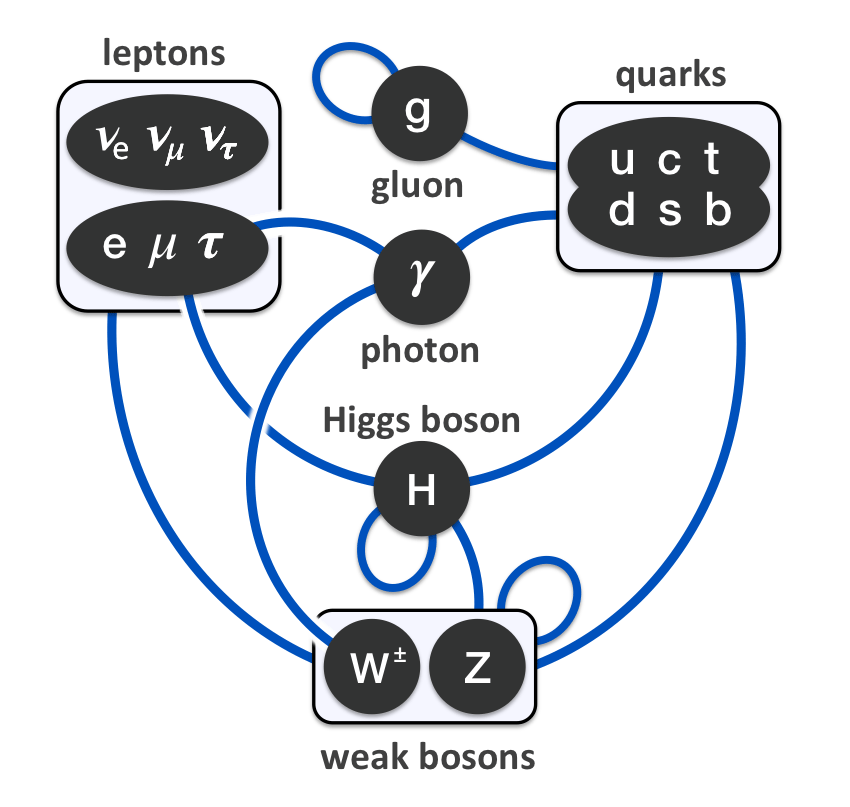
\includegraphics[width=0.75\textwidth]{figures/couplings.png}
  \caption{A diagram of the interactions, or couplings,
    between the particles of the Standard Model. Particles or groups
    of particles connected by blue lines are able to interact with
    each other.}
  \label{fig:couplings}
\end{figure}

\subsubsection*{Force Carriers}
The Standard Model describes four force-carrying particles. These
particles are the physical manifestations, or \emph{quanta}, of the forces
they convey. In general, particles interact with other particles through the
force-carriers. However, not all particles are able to interact with
all forces.

The photon ($\gamma$) is the quantum of the electromagnetic
force. Thus every time two particles interact electrically or
magnetically, they do so by exchanging photons. Only particles that
have a non-zero electric charge can interact electromagnetically. Thus
we say the photon \emph{couples to} charged particles. All quarks, as
well as the charged lepton, carry electric charge. In addition, the
photon is the particle of light. Thus when an object is illuminated by
light, it is actually being bombarded by photons. The photon must
therefore travel at the speed of light, which means it must have zero
mass.

The gluon ($g$) is the carrier of the strong nuclear force. The strong
force is responsible for binding together quarks to form protons,
neutrons, and other composite particles (known collectively as
hadrons). This same interaction also causes protons and neutrons to
bind together and form atomic nuclei. Gluons couple to any particle
that has so-called \emph{color charge}, including quarks, as well as
other gluons. Although gluons are in principle massless, the energy of
their collective interactions actually makes up more than 99\% of the
mass of protons and neutrons.

The W and Z bosons ($W^+, W^-, Z$) carry the weak nuclear force. This
force is best known for mediating radioactive $\beta$-decay through
the W-bosons. In addition, the only way quarks can change flavor is by
interacting via a W-boson, so W-bosons are very commonly produced when
heavier quarks decay into lighter ones.
Particle physicists know the Z-boson best for its
role in the Drell-Yan process, where pairs of quarks convert into
pairs of charged leptons. The W and Z bosons couple to all matter
particles. In addition, they are capable of coupling to each other,
though such interactions are rare. The W bosons have a mass of around
80 GeV, and the Z boson has a mass around 91 GeV \cite{pdg}.

\subsubsection*{Higgs Boson}
The Higgs boson is included here for completeness, and for the benefit
of the curious reader, although it plays
no role in the research described in this dissertation. The Higgs
boson is neither a force-carrying particle nor a matter particle, but
something else entirely. It is the manifestation, or quantum, of the
Higgs field, a field that permeates the entire universe, and endows
mass upon most elementary particles. The top quark is so massive
because it couples very strongly to the Higgs field. Similarly, the
photon is massless because it does not couple to the Higgs field at all.
The Higgs boson itself was discovered to have a mass of about 125 GeV,
which means the Higgs must couple to itself.

\subsubsection*{Antimatter}
For every matter particle, there also exists a corresponding
antiparticle. These are collectively referred to as
antimatter. Antiparticles generally have the exact same properties as
their normal-matter partner, except that their electrical charge (if
they have one) is opposite in sign. Thus the anti-electron (also
called a positron) has a positive electrical charge instead of
negative. The antimatter versions of the charged leptons are indicated
with a plus in their symbol ($e^+, \mu^+, \tau+$), and all other
antiparticles have a bar on top of their symbol ($\bar{u},
\bar{b}, \bar{\nu_{\mu}}$, etc.). When a particle meets its own
antiparticle, they usually produce high-energy photons, or sometimes
Z-bosons. Additionally, quark-antiquark pairs \emph{of different
  flavor} can produce or be produced by W-bosons. Because antimatter
annihilates on contact with normal matter, it is not found
in large quantities in our universe. However, very small quantities can be
produced by energetic particle collisions in nature, and in manmade
particle colliders.

%%%%%%%%%%%%%%%%%%%%%%%%%%%%%%%%%%%%%%%%
% Do I need to explain Feynman diagrams?
%%%%%%%%%%%%%%%%%%%%%%%%%%%%%%%%%%%%%%%%

\subsection{Successes}
\label{ssec:SMsuccesses}

Correctly predicted pretty much every physics result in the last... what, 30 years?

\subsection{Shortcomings}
\label{ssec:SMshortcomings}

Gravity / hierarchy problem
Fine tuning of masses
Higgs mass surprise
Dark Matter
Dark Energy
neutrino masses and oscillations

\section{Supersymmetry}
\label{sec:susy}

Also known as SUSY

\subsection{Motivation}
\label{ssec:susymotivation}

It's possible this part should be split between the preceding and
subsequent sections. Not sure.

\subsection{Principles}
\label{ssec:susyprinciples}

Explain about sparticles, the differences from particles,
the naming conventions, and how they fix some of the problems
of the Standard Model

\subsection{Sparticles}
\label{ssec:susysparticles}

I think this is somewhat redundant. It might wind up fitting more
naturally into the previous section. Or who knows, maybe this entire
section will wind up having NO subsections at all. IDK.

\section{Top quarks as a window to BSM physics}
\label{sec:topquarks}

Explain why the heavy mass of the top quark makes it a natural link
to physics beyond the standard model.